\section{Experimental Evaluation}\label{sec:evaluation}

\subsection{Domains Setup}

%\subsubsection{Domains}

\begin{table}
	\caption{Continuum Setup for the Experimental Evaluation}
	\label{tab:domain-exp-config}
	\begin{tabular*}{1\textwidth}{@{\extracolsep{\fill}}>{\raggedright}p{1.5cm}>{\raggedright}p{6cm}>{\raggedright}p{6cm}}
		\toprule 
		Domain & Machine Resources & Execution Environment\tabularnewline
		\midrule
		\midrule 
		Edge-Local & ubuntu/trusty64-2, 4x vCPUs, 4Gb RAM & Openwhisk, 256 Mb/Action, Python 2.7 + OpenCV \tabularnewline
		\midrule 
		Edge-Mobile & ubuntu/trusty64-2, 8x vCPUs, 16Gb RAM & Openwhisk, 256 Mb/Action, Python 2.7 + OpenCV \tabularnewline
		\midrule 
		Cloud-FaaS & N/A & AWS Lambda, 256 Mb/Function, Python 2.7 + OpenCV \tabularnewline
		\midrule 
		Cloud-IaaS & Autos Scaling Group with t2.micro instances + Amazon Linux AMI 2017  & NodeJs 6.11 server + Python 2.7 + OpenCv \tabularnewline
		\bottomrule
	\end{tabular*}
\end{table}

Table~\ref{tab:domain-exp-config} shows the different domains that were deployed to materialize the computational continuum for the experiments. Edge domains feature the Apache Openwhisk (formerly IBM Openwhisk) serverless framework\footnote{https://openwhisk.incubator.apache.org/} that manages {\em actions} (equivalent to functions). Being open-source, openwhisk is (to date) the only serverless alternative among the major vendors that can be deployed locally or on private clouds. 
%Particularly, openwhisk provides a built-in noSQL database: CouchDB, which is associated with the implemented actions through user-defined triggers and rules. 
Particularly, Edge-local domain is always placed close to the client applications/devices (one or two network hops). This deployment allows us to represent a situation where latency is close to zero, but the computational resources are highly constrained, as scaling-up is not possible due to inherent physical restrictions of the underlying infrastructure. Similarly, the Edge-mobile domain is placed on an university server, where the computational resources are less constrained, and still low latency can be achieved due to physical proximity and data locality. Note that in both cases the domains are deployed in the same LAN that originates the requests, to emulate the few-hop scenario in which devices are directly connected to their nearest Edge domains.


%In this experiment, we considered two alternatives for deploying the serverless continuum architecture, mimicking the behavior of both an edge node and a fog node (Figure~\ref{fig:exp-edge}).  

%The client application is embedded in the edge node, consisting on the postman requests and the node.js endpoint (Figure~\ref{fig:exp-setup1}). 
%On the edge-local alternative, we used a virtual machine running locally, on a regular laptop, with 4x CPU, 4x Gb of RAM and 40 Gb SSD of storage. 

%For the Fog alternative, we deployed the serverless architecture on Policloud\footnote{http://policloud.polimi.it/}, the private IaaS solution of Politecnico di Milano. Here, the computational resources are less constrained, and still low latency can be achieved due to physical proximity (two hops from the client) and data locality. This setup runs on a small cluster of 4 virtual machines with 2x CPU, 4x Gb of Ram and 100 GB SSD, each running a different component of openwhisk (triggers and storage, Http server, controller, and invokers, respectively). Note that in this case the fog node is deployed in the same LAN that originates the requests, to emulate the few-hop scenario in which devices are directly connected to their corresponding MEC.

The serverless cloud alternative (Cloud-FaaS) for this experiment uses AWS Lambda\footnote{https://aws.amazon.com/lambda/} as the first-available and most mature serverless solution in the market. The functions and associated libraries and services (storage, image recognition) are hosted in the same region, which is enforced by AWS to guarantee a certain degree of data locality. Finally, we also deployed the feature recognition functionality as a ``serverful'' Cloud setup (Cloud-IaaS). However, the main goal of this experiment is not to compare traditional cloud services against a serverless solution, but to demonstrate that the proposed continuum can outperform the Cloud under certain circumstances and requirements.


\subsection{Domain Latency Evaluation} 

In order to compare the latency along the continuum, we performed experiments with different number of parallel requests firing at a constant rate. Each request consisted on feature extraction and matching from a sample image. This experiment was performed without using the A3-E middleware, since it aims to evaluate only the different domains.

Figure~\ref{fig:exp-setup1} shows the experimental setup. Capturing and uploading an image is emulated using Postman\footnote{https://www.getpostman.com/}, a JavaScript open source application designed to load test functional behaviors and measure the performance of Web APIs. The  payload for this experiment was a sample image of approximately 65 Kb, which is a reasonable size for this use case considering the requirements regarding low-latency, computation time and battery consumption~\cite{rodriguez16mobile}. 

Then, the image is sent through HTTP/POST and different subsequent steps are executed depending on the domain: Openwhisk actions for both Edge domains, AWS Lambda functions for Cloud-FaaS domain, and a simple Nodejs server that calls a Python function for Cloud-IaaS domain.

%In our edge domains for the experiment, uploading an image to CouchDB (Step 3.a) triggers the action that performs the feature extraction and matching (Step 4.a)  with the points-of-interest, supported by the OpenCV\footnote{\url{http://opencv.org}} visual recognition library (Step 5.a). 


\begin{figure}
	
	\centering
	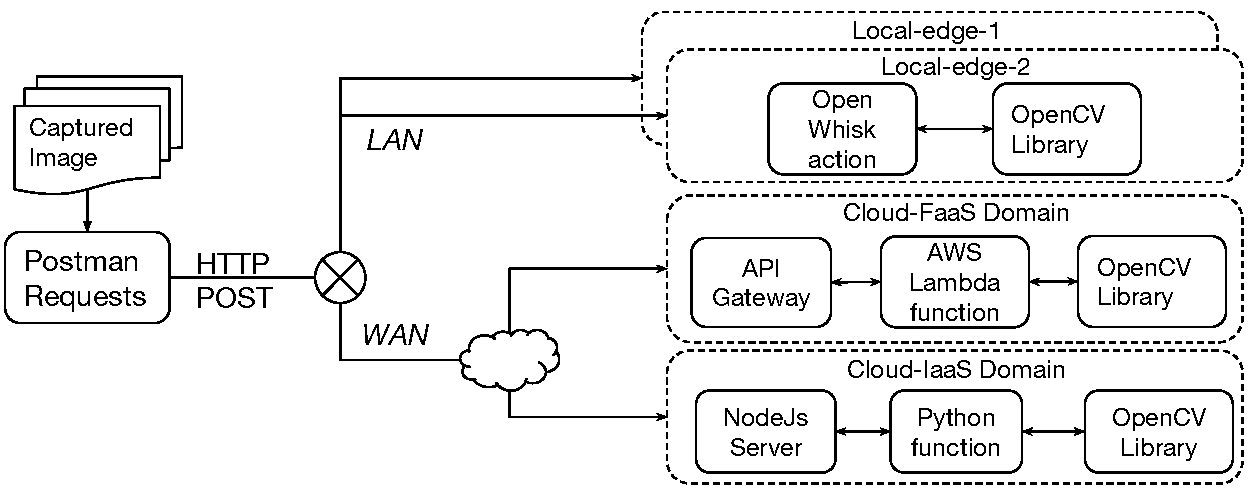
\includegraphics[width=0.9\textwidth]{figs/experimental-setup.pdf}
	\caption{Setup for Latency Experiments}
	\label{fig:exp-setup1}
\end{figure}

%\subsubsection{Baseline Latency}

To measure the latency, the workload was parameterized using different number of parallel clients, which perform 100 requests each, fired at a constant rate of two per second. This setup considers not only the default maximum for concurrent executions in AWS Lambda\footnote{http://docs.aws.amazon.com/lambda/latest/dg/concurrent-executions.html} and Openwhisk\footnote{https://github.com/apache/incubator-openwhisk/blob/master/docs/reference.md}, but also the limited resources of the edge domains. 

The experiment stresses progressively the different domains, and allows to compare the relative latency under each workload. Figure~\ref{fig:latency-domains} shows the average latency for each scenario, averaged through 5 executions. Note that the function computation time (light gray) is distinguished from the overhead (dark gray), which includes network communication (routing, forwarding) and queuing time (when no resources are available to process the request immediately). 

\begin{figure}
	
	\centering
	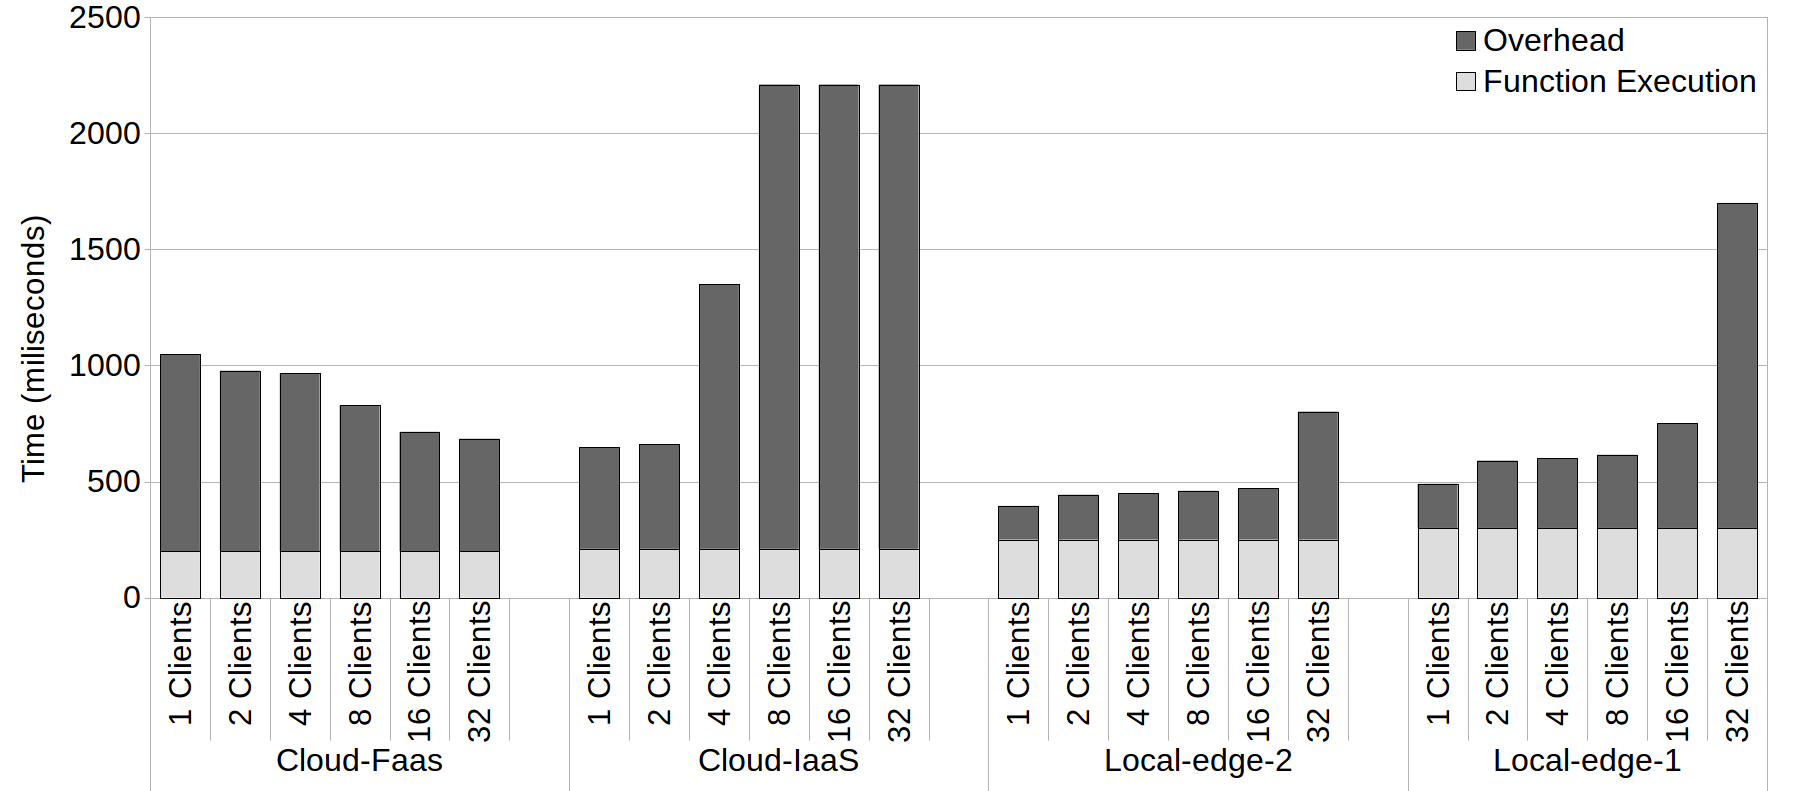
\includegraphics[width=1\textwidth]{figs/latency-domains}
	\caption{Latency results for each domain and different number of clients.}
	\label{fig:latency-domains}
\end{figure}

 For these scenarios, the latency added by the edge domains is less than the latency in both cloud alternatives, considering up to 16 simultaneous clients, with a rate of 2 $requests/second$ each. Regarding the serverless cloud alternative, the overhead reduction is up to 90\% for edge-local and up to 82\% for edge-mobile respectively. Regarding the traditional cloud domain, reductions are up to 77\% and 58\% respectively. Since a scaling-up action triggers when more than one VM instance is needed to handle the workload (that can demand several seconds~\cite{Quatrocchi2016discrete}), requests timeout in the meantime. 
 
 For light to medium workloads, the edge-local and edge-mobile domains outperformed all the other alternatives for this scenario. However, edge-local domain is the most resource-constrained, which hinders its availability under heavier workloads. Interestingly, the traditional cloud domain also outperformed the serverless one (46\% less latency) for light workloads. This can be due to the additional steps performed by the API Gateway in order to forward RESTful calls to lambda functions\footnote{http://docs.aws.amazon.com/lambda/latest/dg/with-on-demand-https.html}. Nevertheless, this advantage is mitigated by the fact that the serverless alternative is more reactive against bursts of workload, scaling faster and offering a fine-grained cost model~\cite{Villamizar2017lambda,Hendrickson:2016}.


%\subsection{Battery} The second set of experiments targeted the measurement of battery consumption of a mobile device in two scenarios: 1) in which feature extraction and matching were performed locally, and 2) these tasks were offloaded to edge servers.

\subsection{Continuum} The next set of experiments targeted the evaluation of A3-E with a computational continuum scenario. In specific, the evaluation consisted of a mobile device hosting a simplified version of an AR application with the feature extraction and matching modeled as stateless functions that can be executed locally (Java Functions), in an edge-based FaaS platform (OpenWhisk), or a cloud-based FaaS platform (Amazon Lambda). We measured the following parameters: Battery consumption, total execution time, and time per call. The experiment featured four different scenarios: With only one domain available (either locally in the device, edge-mobile or cloud-faas), and then with all domains available at the same time (all-domains). \textcolor{blue}{[TODO] (1) Explain the probabilities of having each domain available. (2) Discuss the relevance of the results} 
Figure~\ref{fig:exp-a3e} shows the results for the experiment, averaged among 5 executions for each scenario.

\begin{figure}[tbp]
	\raggedright
	\subfloat[Battery consumption (\%)\label{fig:battery-a3e}] {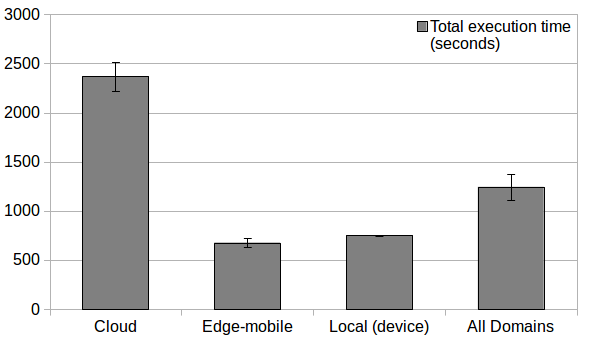
\includegraphics[width=0.5\textwidth]{figs/total-exec-time-A3E}}
	\subfloat[Total execution time (seconds)\label{fig:total-exec-a3e}] {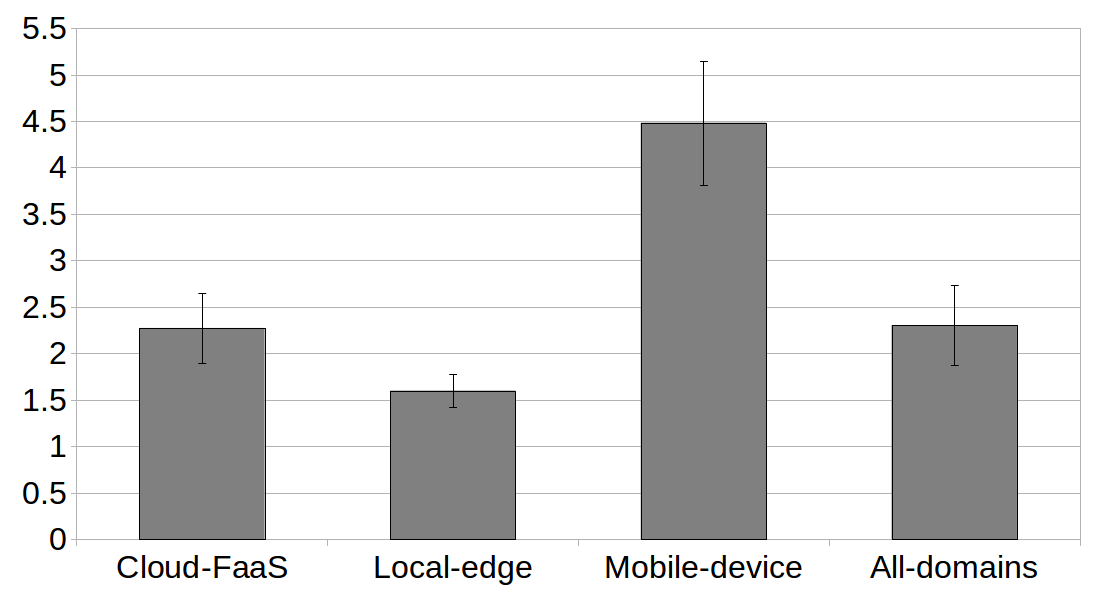
\includegraphics[width=0.5\textwidth]{figs/battery-consumption-A3E}}
	
	\centering\subfloat[Execution time per call (miliseconds)\label{fig:time-per-call-a3e}] {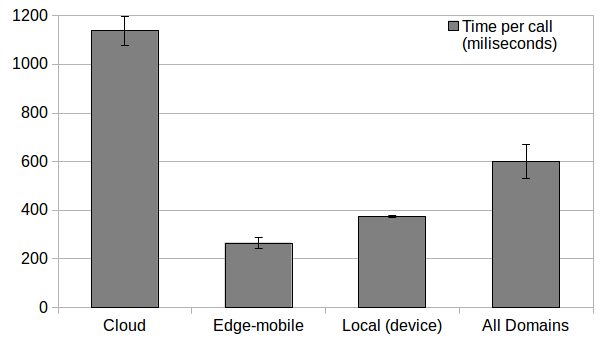
\includegraphics[width=0.5\textwidth]{figs/time-per-call-A3E}}

	\caption{A3-E experimental evaluation results} \label{fig:exp-a3e}
\end{figure}





